\section{Edward}
This is the section dedicated to Edward, and it was written individually . It includes a range of things; the first subsection is a space pointing out the strengths and weaknesses of the module, including complaints about the module coordinator Max Wilson. The second section is a selfie image with Max! The last part of it is the most important one. It is a paragraph about what Edward has learned in this module. 

Please do not forget:
\begin{itemize}
	\item First paragraph should have your comments about the module
	\item Second one, a selfie img with Max
	\item Last one, what you learned in this module.
\end{itemize}

\subsection{Comments about the module}
The best part of this module is working in a team as it allows me to blame others for my own mistakes.

\subsection{Selfie with Max}

To include an image, you will need to remove the comments from the code below, place an image in the main folder, and do not forget to put the name of the image instead of ImgName. 

\begin{figure}[h]
\caption{Selfie with Max}
\centering
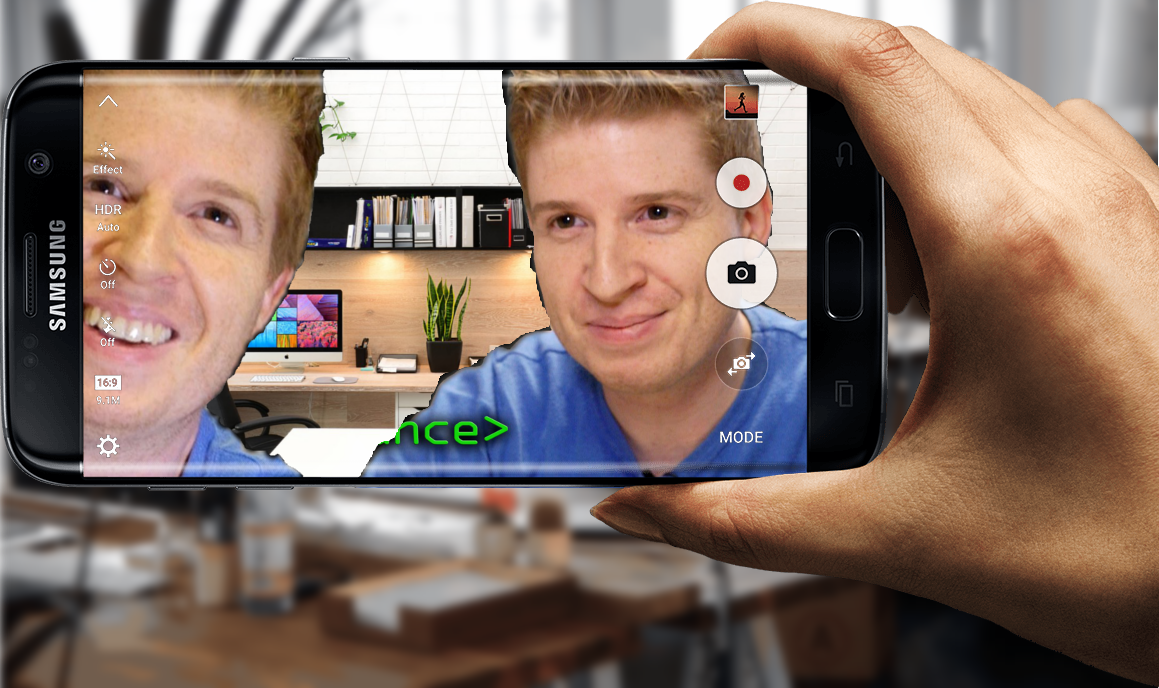
\includegraphics[width=0.5\textwidth]{images/mastapeece.png}
\label{fig:selfie}
\end{figure}

You can then use the label of the figure to reference it later with the command ${\backslash}ref$. you can comment out the next line to see an example of how it works.

% My selfie with Max is in  Figure~\ref{fig:selfie}.

\subsection{What I have learned in this module}
I have learnt an awful lot about the dos and don'ts of software engineering. 

